\subsubsection{Read}
\begin{figure}[H]
\centering
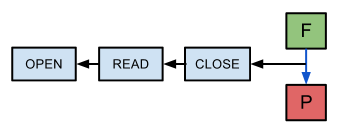
\includegraphics[scale=0.5]{res/sem/R.png}
\caption{Read Semantics}
\label{fig:rsem}
\end{figure}

During a read operation, a link is created from the file being read to the process that has opened the file for reading. The list of I/O operations performed are added as a chain to the file and process provenance records. The data for the I/O chain is stored in a separate database and each node in the chain has a unique I/O ID.

\subsubsection{Create}
\begin{figure}[H]
\centering
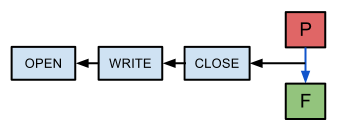
\includegraphics[scale=0.5]{res/sem/W.png}
\caption{Create Semantics}
\label{fig:wsem}
\end{figure}

When a process opens a file in write mode with the create flag, a link will be created from the process to the file. The I/O chain common to the process and file will show the list I/O operations performed.

\subsubsection{Append}
\begin{figure}[H]
\centering
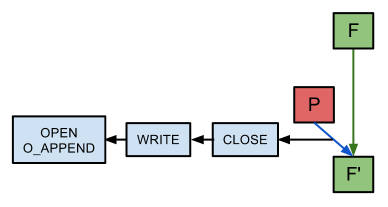
\includegraphics[scale=0.5]{res/sem/A.png}
\caption{Append Semantics}
\label{fig:asem}
\end{figure}

When a process opens a file in append mode, the file pointer is automatically set to the end of the file. Any data written by a process to the file is appended to the existing contents in the file. A file provenance record and a process provenance record are generated as shown in figure \ref{fig:asem}. A link from the file's previous provenance record is connected to the new file provenance record. An I/O chain is added to the process and file provenance records.


\subsubsection{Read and Append}
\begin{figure}[H]
\centering
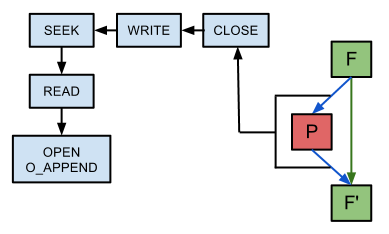
\includegraphics[scale=0.5]{res/sem/RandA.png}
\caption{Read and Append Semantics}
\label{fig:randasem}
\end{figure}

When a file is opened in read and append mode, the initial file position for reading is at the beginning of the file, however any data written is appended to the end of the file. A new provenance record is created for the file being appended. Links from both the process and the old file provenance records point to the new file provenance record. The I/O chain generated during this process is common to the process and file entities as shown in figure \ref{fig:randasem}.

\subsubsection{Truncate}
\begin{figure}[H]
\centering
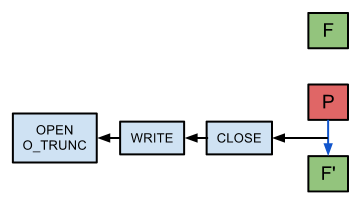
\includegraphics[scale=0.5]{res/sem/T.png}
\caption{Truncate Semantics}
\label{fig:tsem}
\end{figure}

When a file is opened with the truncate flag set or if a file is opened in write mode and a truncate function call is made to erase the contents of the file, a new file provenance record is created as shown in figure \ref{fig:tsem}. There is no link from the old file provenance record to the new file provenance record as the file contents are completely destroyed. The I/O chain created is common to the process and the new file provenance record.

\subsubsection{Rename}
\begin{figure}[H]
\centering
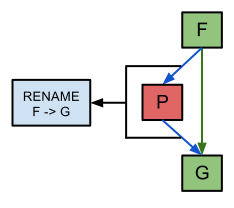
\includegraphics[scale=0.5]{res/sem/rename.png}
\caption{Rename Semantics}
\label{fig:rensem}
\end{figure}

When a file is renamed, a new provenance record is created as shown in figure \ref{fig:rensem}. As the content of the old file is preserved in the new file, a link is made from the old file to the new file provenance record. The I/O chain is common to both the process and file provenance records.

\subsubsection{Unlink}
\begin{figure}[H]
\centering
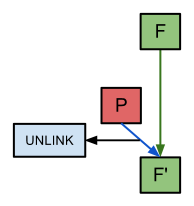
\includegraphics[scale=0.5]{res/sem/unlink.png}
\caption{Unlink Semantics}
\label{fig:usem}
\end{figure}

During an unlink operation on a file, a new file provenance record is created and the I/O chain contains details of the unlink function call that was made. A link from the old file provenance record to the new file provenance record is created.
